\documentclass[a4paper,12pt]{article}
\usepackage{graphicx}  % For including images
\usepackage{amsmath}   % For mathematical symbols
\usepackage{amssymb}   % Additional math symbols
\usepackage{hyperref}  % For hyperlinks
\usepackage{xcolor}    % For colored text
\usepackage{listings}  % For code formatting
\usepackage{caption} % For customizing captions
\usepackage{float} % For positioning figures
\usepackage{setspace}

\title{\textbf{Digital Signal Processing Lab Report}}  
\author{Eazdan Mostafa Rafin \\ CSE, RUET \\ March 27, 2025}
\date{}

\begin{document}

\maketitle

\section*{Objectives}
\begin{itemize}
    \item Understand basic signal operations.
    \item Implement Discrete Fourier Transform (DFT) manually and compare it with NumPy FFT.
    \item Compute Discrete-Time Fourier Transform (DTFT).
    \item Analyze the efficiency of Fast Fourier Transform (FFT).
    \item Apply filtering in the frequency domain.
\end{itemize}

\section*{Problem Statement}
In these set of lab problems, we will explore key concepts in Digital Signal Processing (DSP) by working with signals, Fourier transforms, and filtering techniques. We will start by generating discrete-time signals and modifying them through shifting, scaling, and reversal. Then, we will implement the Discrete Fourier Transform (DFT) from scratch and compare it with NumPy’s built-in FFT function to understand efficiency differences. We will also analyze signals using the Discrete-Time Fourier Transform (DTFT) and apply a low-pass filter to remove unwanted high-frequency noise.

\section*{Theoretical Background}
\subsection*{Basic Signal Operations}
- Time Shifting: $x[n - k]$  \\ 
  Time shifting involves shifting a signal in time without altering its shape. A positive shift moves the signal to the right, while a negative shift moves it to the left. \\
  \\
- Time Reversal: $x[-n]$ \\
  Time reversal flips the signal about the vertical axis, effectively reversing its sequence.\\
  \\
- Time Scaling: $x[a \cdot n]$ \\
  Scaling a signal compresses or stretches it. When $a > 1$, the signal is compressed; when $0 < a < 1$, the signal is stretched.

\subsection*{Fourier Transforms}
\subsubsection*{Discrete Fourier Transform (DFT)}
The Discrete Fourier Transform (DFT) converts a discrete-time signal from the time domain to the frequency domain. It is mathematically defined as:
\begin{equation}
    X[k] = \sum_{n=0}^{N-1} x[n] e^{-j \frac{2\pi}{N} kn}
\end{equation}
DFT provides frequency domain representation but has high computational complexity, making it inefficient for large $N$. The Fast Fourier Transform (FFT) is an optimized algorithm to compute the DFT efficiently.

\subsubsection*{Discrete-Time Fourier Transform (DTFT)}
Unlike the DFT, which is limited to a finite number of frequency components, the DTFT is a continuous function of frequency:
\begin{equation}
    X(e^{j\omega}) = \sum_{n=-\infty}^{\infty} x[n] e^{-j\omega n}
\end{equation}
The DTFT provides a more precise representation of frequency content but requires infinite summation, making it theoretical rather than computational.

\subsection*{Fast Fourier Transform (FFT) Efficiency}
The FFT is an efficient algorithm to compute the DFT in $O(N \log N)$ time complexity instead of $O(N^2)$. This significantly reduces the computational load, especially for real-time signal processing applications.

\subsection*{Filtering in the Frequency Domain}
Filtering in the frequency domain involves manipulating the frequency components of a signal. A low-pass filter allows only low-frequency components to pass while attenuating high-frequency components. This is useful for removing noise and smoothing signals.

\section*{Implementation Process}
\subsection*{Signal Generation and Transformations}
\begin{enumerate}
    \item Generate a discrete-time sine wave using NumPy.
    \item Perform time shifting by delaying or advancing the signal.
    \item Perform time reversal by flipping the signal indices.
    \item Perform time scaling by compressing or expanding the signal in time.
\end{enumerate}

\subsection*{Discrete Fourier Transform (DFT)}
\begin{enumerate}
    \item Implement the DFT manually using the mathematical formula.
    \item Compute the DFT using NumPy's built-in FFT function.
    \item Compare results to verify accuracy.
\end{enumerate}

\subsection*{Discrete-Time Fourier Transform (DTFT)}
\begin{enumerate}
    \item Compute the DTFT by evaluating the Fourier transform for a range of frequencies.
    \item Plot the magnitude and phase response.
\end{enumerate}

\subsection*{Fast Fourier Transform (FFT) Efficiency}
\begin{enumerate}
    \item Measure execution time for manual DFT.
    \item Measure execution time for FFT.
    \item Compare and analyze the speed difference.
\end{enumerate}

\subsection*{Filtering in the Frequency Domain}
\begin{enumerate}
    \item Apply FFT to transform the signal to the frequency domain.
    \item Design a low-pass filter to retain only low frequencies.
    \item Apply the inverse FFT to transform the signal back to the time domain.
\end{enumerate}

\section*{Code Implementation}
\subsection*{Basic Signal Operations (Signal Generation and Transformations)}
\textbf{Python Code:}
\begin{lstlisting}[language=Python, caption=Signal Generation and Transformations]
# Sine Wave
def generate_sine_wave(A, f, n, fs):
    return A * np.sin(2 * np.pi * f * n / fs)

x_original = generate_sine_wave(A, f, n, fs)

# Time Shifting
def time_shift(x, k):
    shifted_signal = np.zeros_like(x)
    if k >= 0:
        shifted_signal[k:] = x[:-k] if k > 0 else x
    else:
        shifted_signal[:k] = x[-k:]
    return shifted_signal

# Time Reversal
def time_reversal(x):
    return x[::-1]

# Time Scaling
def time_scaling(x, a):
    n_original = np.arange(len(x))
    n_scaled = n_original * a
    scaled_signal = np.interp(n_original, n_scaled, x)
    return scaled_signal    
\end{lstlisting}

\textbf{Output:}
\begin{figure}[H]
    \centering
    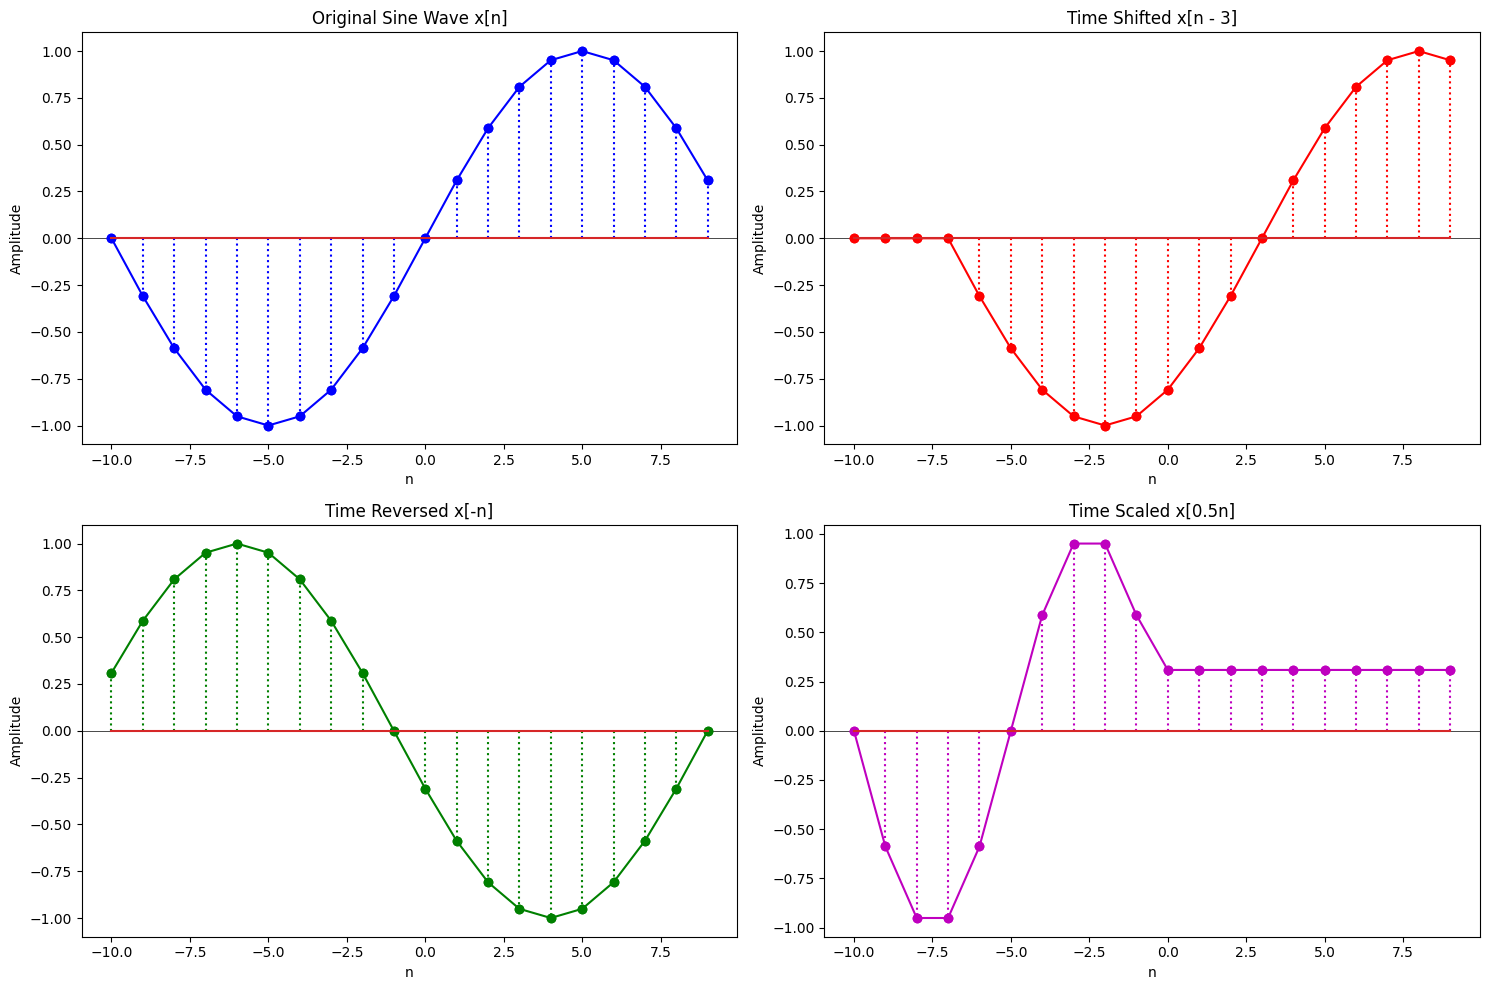
\includegraphics[width=0.8\linewidth]{2.png}
    \caption{Visualization of signal transformations}
    \label{fig:signal_transform}
\end{figure}

\subsection*{Discrete Fourier Transform (DFT)}

\textbf{Python Code:}
\begin{lstlisting}[language=Python, caption=DFT Implementation]
# Manual DFT
def manual_dft(x):
    N = len(x)
    X = np.zeros(N, dtype=complex)

    for k in range(N):
        for n in range(N):
            a = -2 * math.pi * k * n / N
            X[k] += x[n] * complex(math.cos(a), math.sin(a))

    return X

#  DFT Comparison between Manual DFT & Numpy DFT
x = [1, 2, 5, 3, 7]

# Perform DFT comparison
X_manual = manual_dft(x)
# Using Numpy
X_numpy = np.fft.fft(x)
\end{lstlisting}

\textbf{Output:}
\begin{figure}[h]
    \centering
    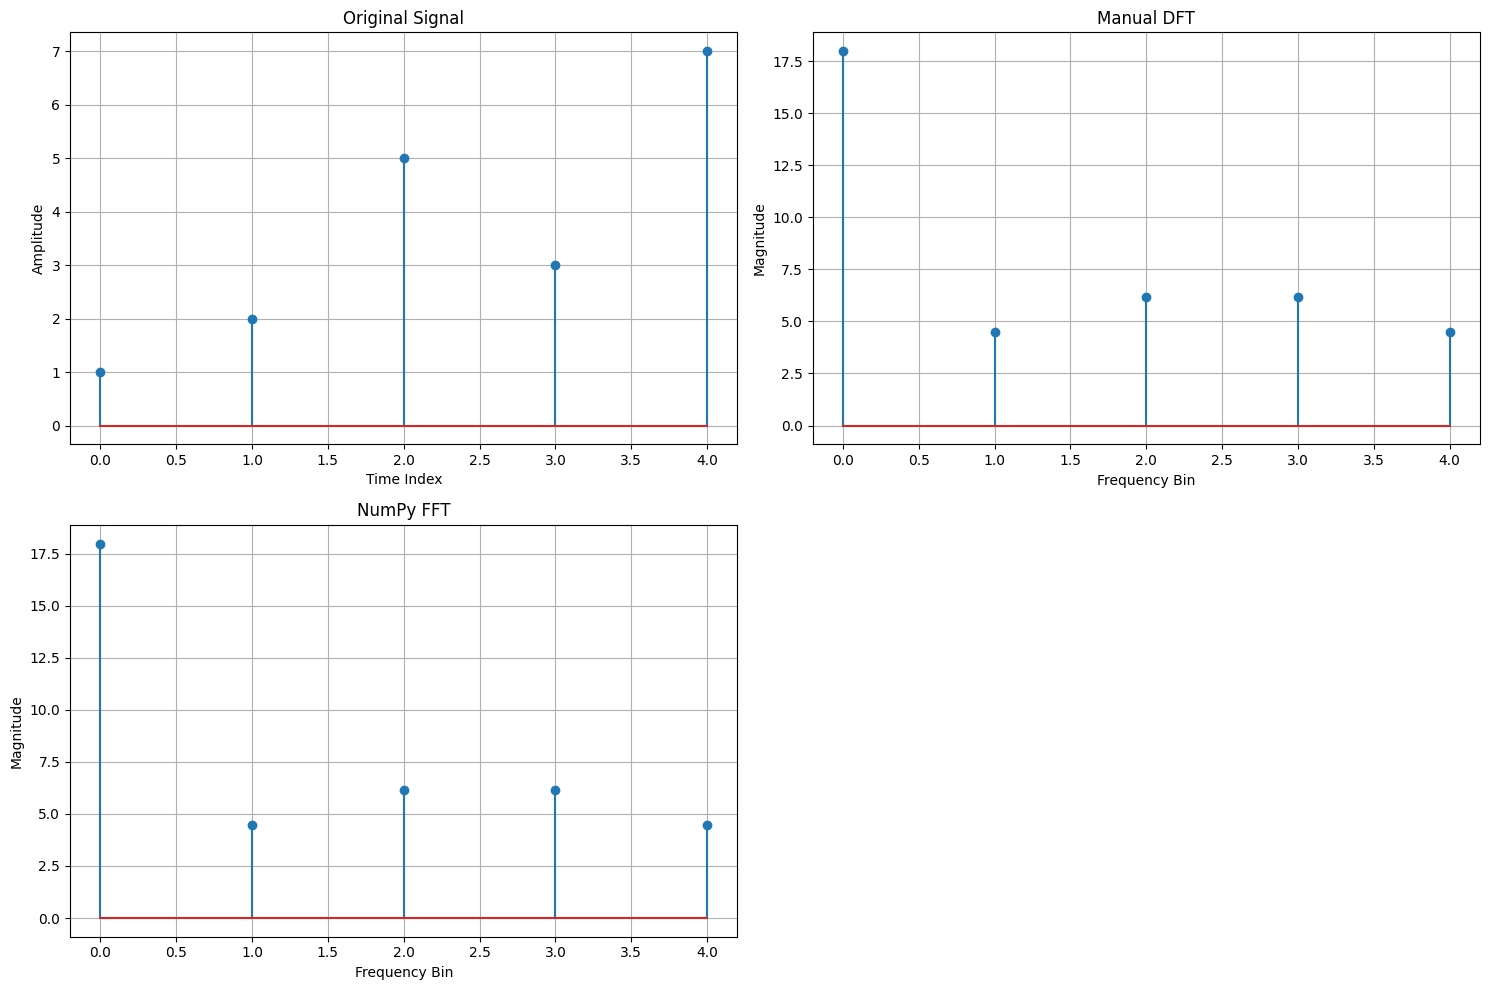
\includegraphics[width=0.8\linewidth]{3.png}
    \caption{DFT vs. FFT comparison}
    \label{fig:dft_vs_fft}
\end{figure}

\subsection*{Discrete-Time Fourier Transform (DTFT)}
\textbf{Python Code:}
\begin{lstlisting}[language=Python, caption=DTFT Computation]
# DTFT Function
def compute_dtft(x, omega):
    X = np.zeros(len(omega), dtype=complex)

    # Compute DTFT using nested loops
    for i, w in enumerate(omega):
        for n in range(len(x)):
            X[i] += x[n] * np.exp(-1j * w * n)

    return X

#Signal
x = np.array([1, 2, 3, 4, 5])
#Frequency range
omega = np.linspace(-np.pi, np.pi, 500)
#DTFT
X_dtft = compute_dtft(x, omega)
\end{lstlisting}

\textbf{Output:}
\begin{figure}[h]
    \centering
    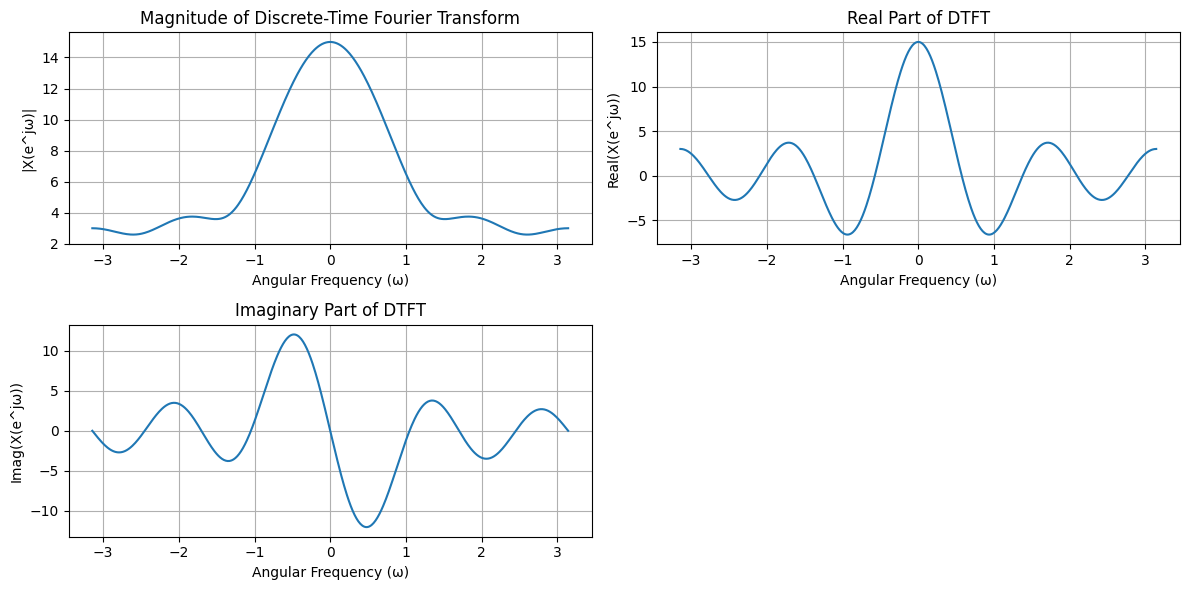
\includegraphics[width=0.8\textwidth]{4.png}
    \caption{DTFT Magnitude}
    \label{fig:dtft}
\end{figure}

\subsection*{Fast Fourier Transform (FFT) Efficiency}

\textbf{Python Code:}
\begin{lstlisting}[language=Python, caption=FFT Efficiency Comparison]
# Fast Fourier Transform (FFT) Efficiency
def time_dft_comparison(signal_sizes=[10, 100, 500, 1000, 2000]):
    manual_times = []
    numpy_times = []

    for size in signal_sizes:
        # Create random signal
        x = np.random.rand(size)

        # Time manual DFT
        start = time.time()
        manual_dft(x)
        manual_time = time.time() - start
        manual_times.append(manual_time)

        # Time NumPy FFT
        start = time.time()
        np.fft.fft(x)
        numpy_time = time.time() - start
        numpy_times.append(numpy_time)

    return manual_times, numpy_times, signal_sizes

# Run time comparison
manual_times, numpy_times, signal_sizes = time_dft_comparison()
    
# Print results
print("Signal Size | Manual DFT Time (s) | NumPy FFT Time (s)")
print("-" * 50)
for size, manual_time, numpy_time in zip(signal_sizes, manual_times, numpy_times):
print(f"{size:10d} | {manual_time:16.6f} | {numpy_time:16.6f}")
\end{lstlisting}

\textbf{Output:}
\begin{figure}[h]
    \centering
    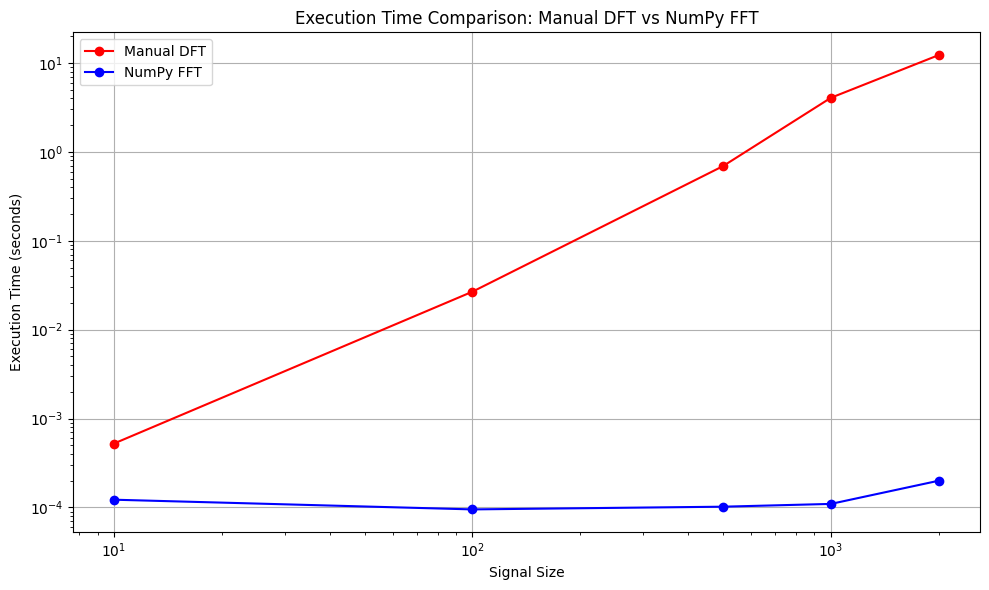
\includegraphics[width=0.8\textwidth]{5.png}
    \caption{Execution Time Comparison}
    \label{fig:fft_efficiency}
\end{figure}

\subsection*{Filtering in the Frequency Domain}

\textbf{Python Code:}
\begin{lstlisting}[language=Python, caption=Low-pass Filtering]
# Noisy signal
n = np.arange(0, 128)
    
# Original signal components
x_signal = np.sin(2 * np.pi * 5 * n / 128)  # 5 Hz
x_noise = 0.5 * np.sin(2 * np.pi * 50 * n / 128)  # 50 Hz
    
# Combining signals
x_noisy = x_signal + x_noise
# Apply low-pass filter in frequency domain
X_fft = np.fft.fft(x_noisy)
frequencies = np.fft.fftfreq(len(n), d=1/128)

# Cutoff Frequency = 10 Hz
H = np.abs(frequencies) <= 10

# Apply the filter
X_filtered = X_fft * H

x_filtered = np.fft.ifft(X_filtered).real
\end{lstlisting}

\textbf{Output:}
\begin{figure}[h]
    \centering
    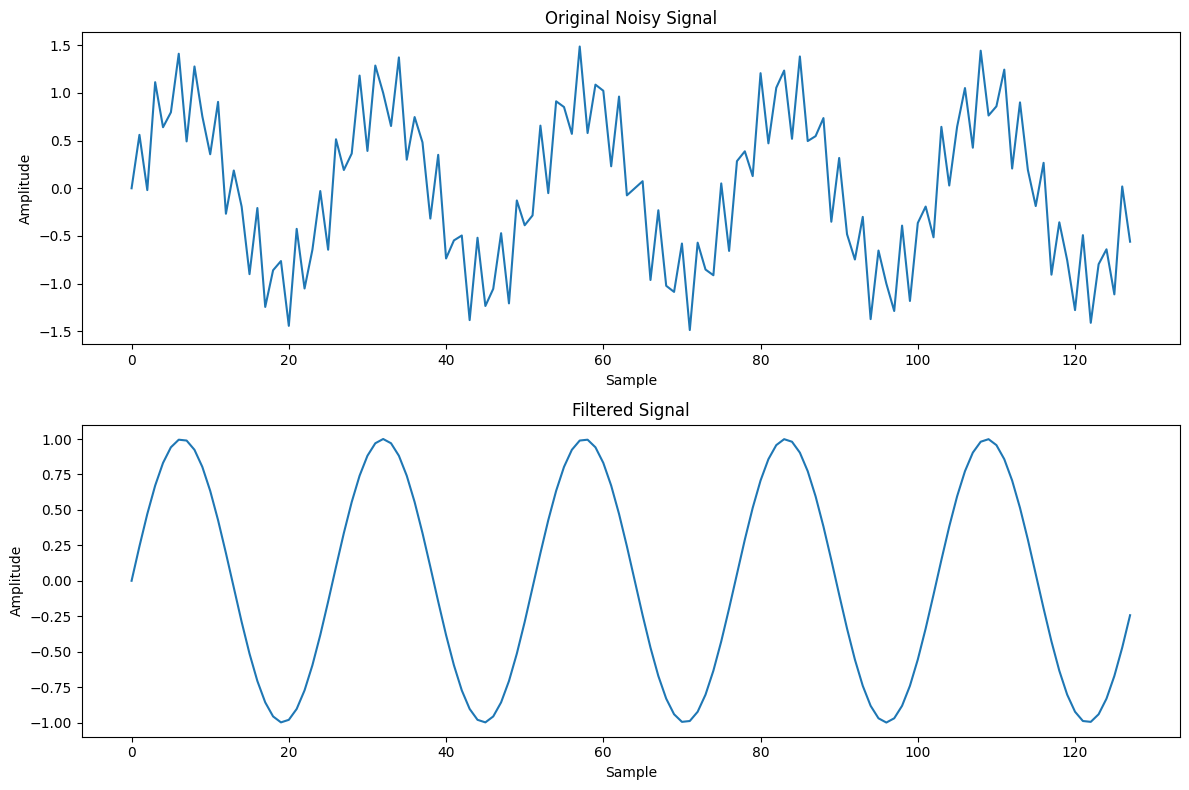
\includegraphics[width=0.8\textwidth]{6.png}
    \caption{Filtered Signal}
    \label{fig:filtered_signal}
\end{figure}

\section*{Conclusion}
These set of experiments explore signal operations, Fourier transforms, and frequency domain filtering, using Python for validation. The FFT proved significantly more efficient than manual DFT, while DTFT reinforced theoretical insights. Low-pass filtering effectively removed noise, demonstrating practical applications of spectral analysis. These experiments highlight the importance of Fourier techniques in signal processing.

\end{document}
